\xsection{myblue}{Optimization}

\begin{frame}{Optimization - Setup}
  \begin{columns}[c,onlytextwidth]
  \begin{column}{0.55\textwidth}
  BRs from minimization through {\color{llblue}\href{https://github.com/scikit-hep/iminuit}{iminuit}}.
  \begin{itemize}
    \item $\vec{S} = M \cdot \vec{B} = \vec{f}(\vec{B})$, with
    \begin{itemize}
        \item $\vec{S}$: The signal counts per category ($S = data - bkg$).
        \item $M$: The matrix build from simulated events, as outlined above.
        \item $\vec{B}$: The target. Use the BRs in the simulation as starting values.
    \end{itemize}
    %\item The cost function: Currently Least Squares.
    %\begin{itemize}
    %    \item $S$: The 1$\sigma$ binomial uncertainties on $S$ are the (only) place where the integrated luminosity effects the analysis.
    %    \item $M$:  Least Squares is not ideal: We discard known information (the total number of events in the sample).
    %\end{itemize}
     \item The cost function: Multinomial log-likelihood.
    \begin{itemize}
        \item $\tn{ln}\mathcal{L} = - N_{\tn{data}} \sum_i S_i \tn{ln}\left(\sum_j M_{ij}B_j\right)$.
        \item $B_{H \to ZZ^*} = 1 - \sum_{i \neq H \to ZZ^*} B_i$.
        \item Each BR constrained to $\left[0, 1\right]$.
    \end{itemize}
  \end{itemize}
  \end{column}
  \begin{column}{0.45\textwidth}
  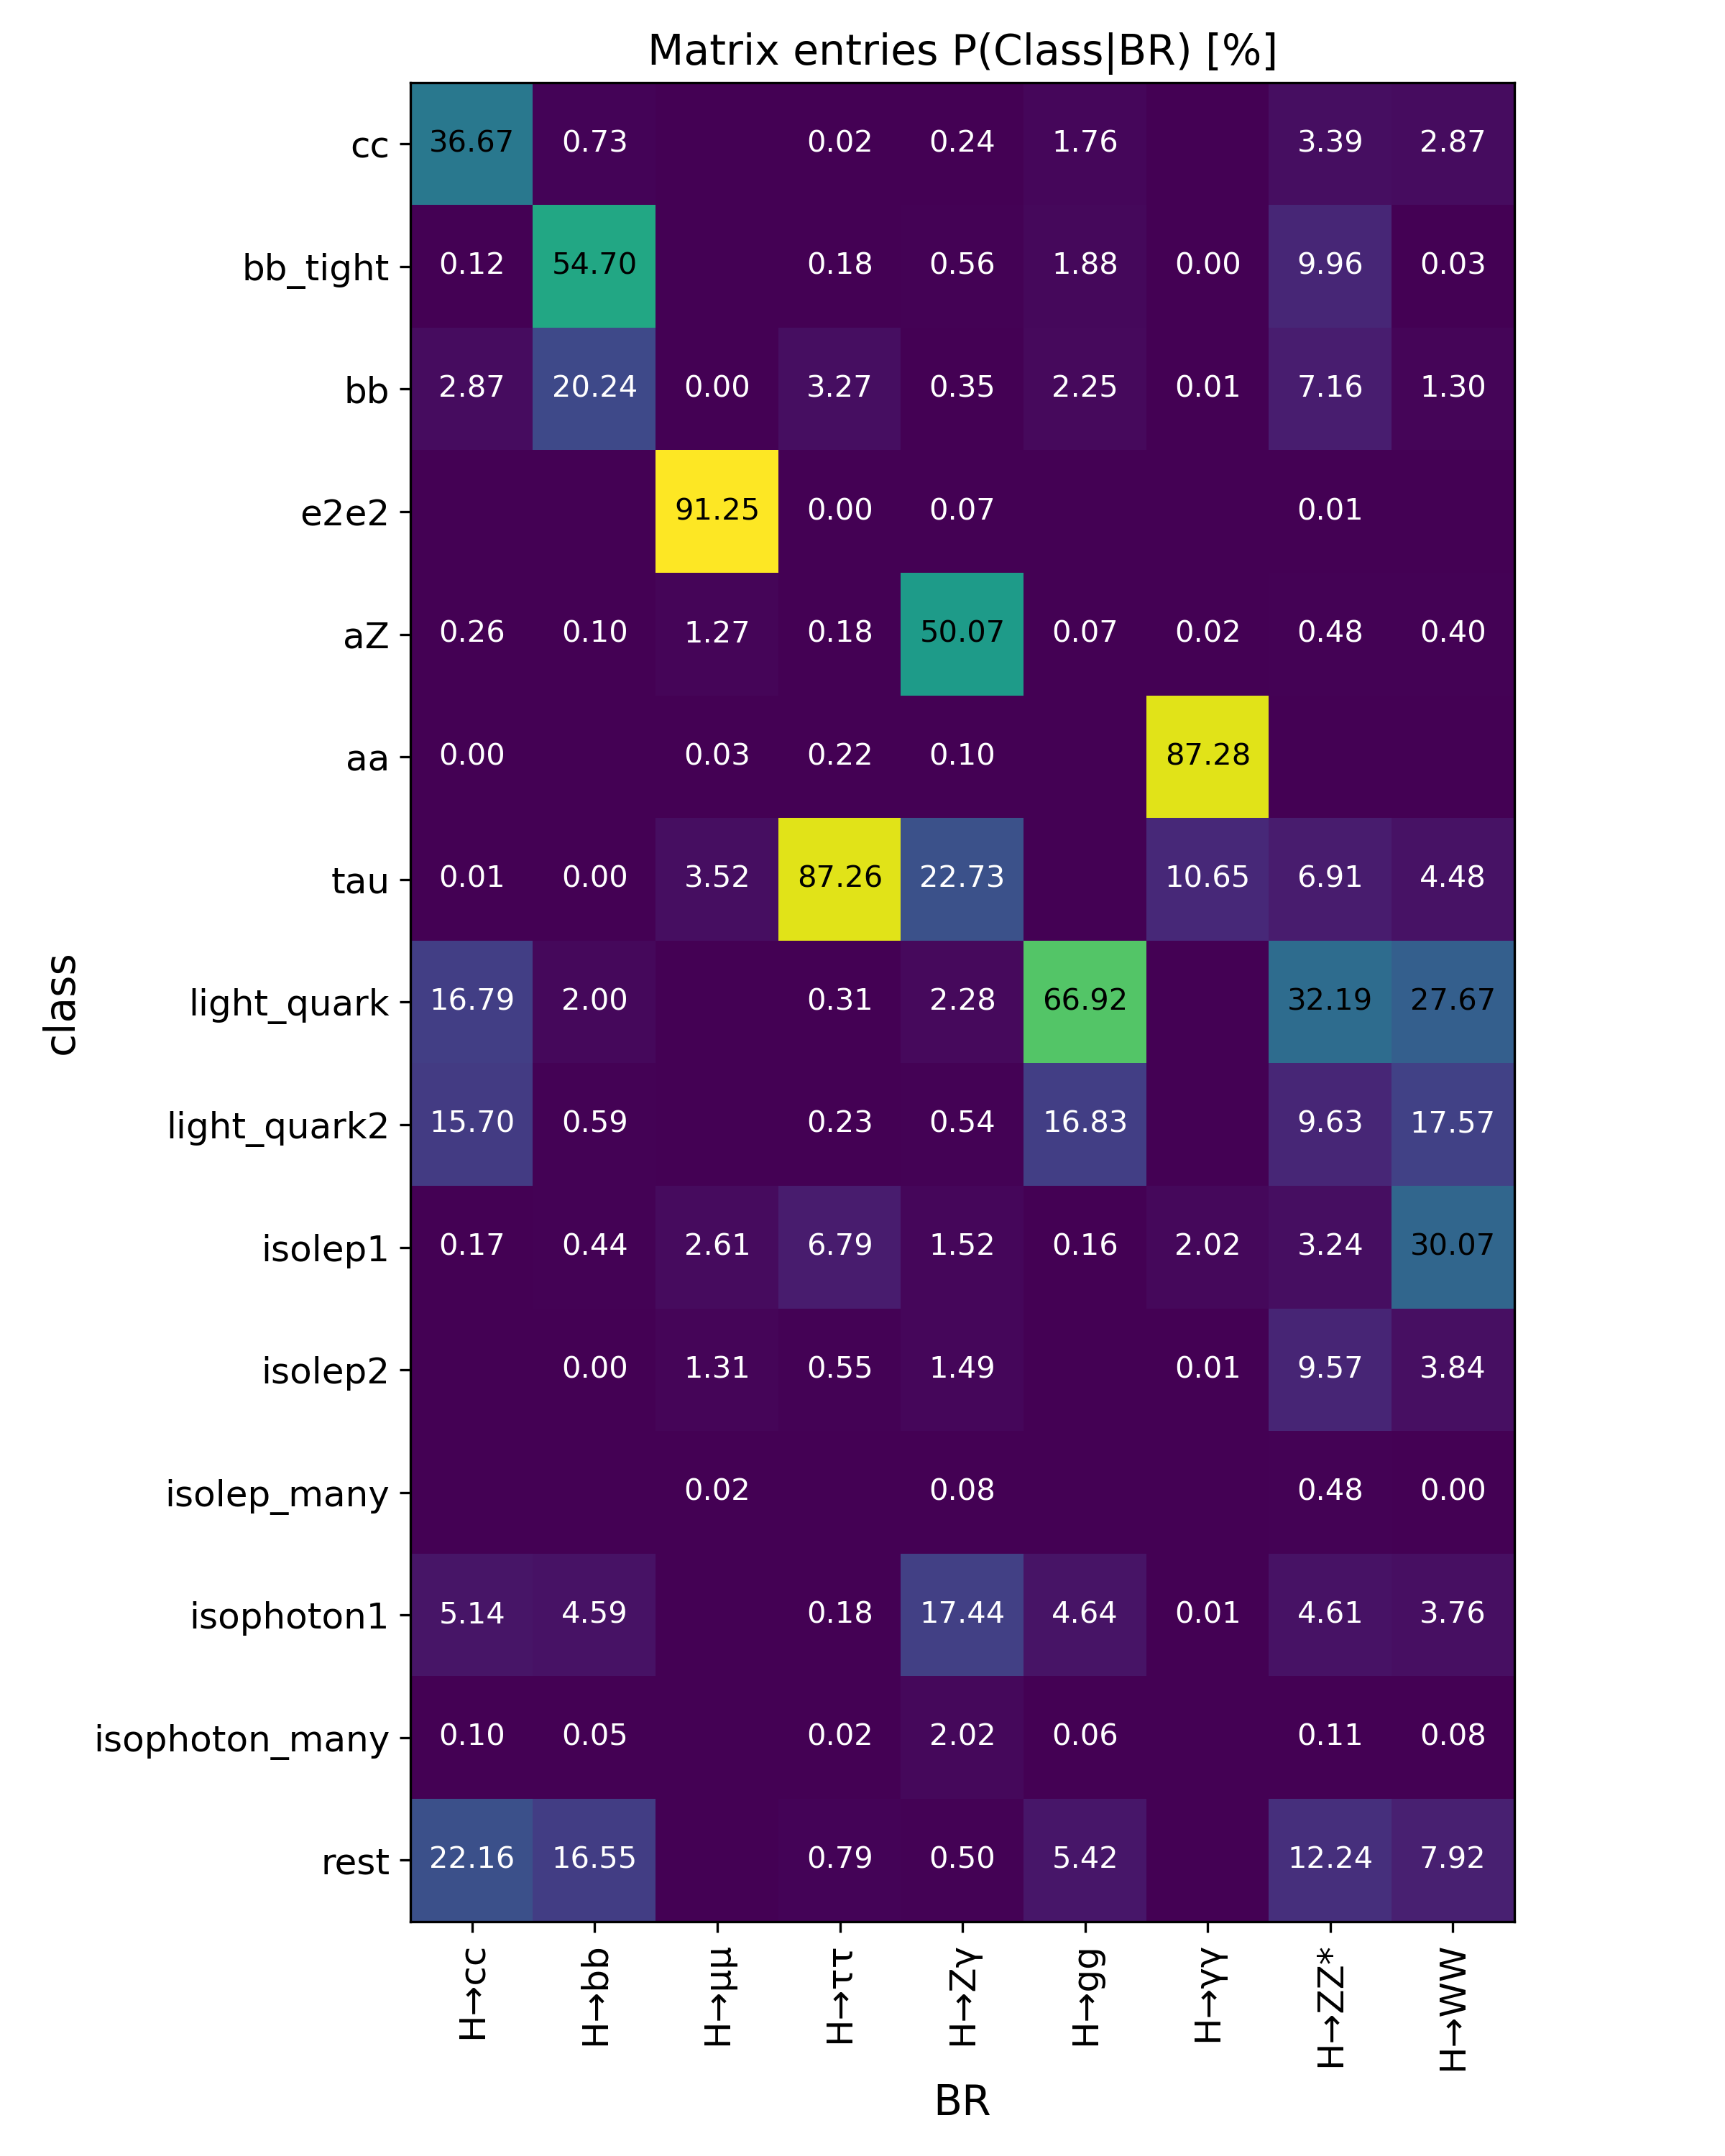
\includegraphics[height=0.9\textheight, width=0.95\textwidth]
      {plot_factory/overlay_free_probability_matrix}
  \end{column}
  \end{columns}
  \end{frame}

\begin{frame}{Optimization - Results}
  \begin{columns}[c, onlytextwidth]
  \begin{column}{0.6\textwidth}
  The fitted BR$^{\tn{min}}$ reproduces BR$^{\tn{true}}$ within its uncertainties.

  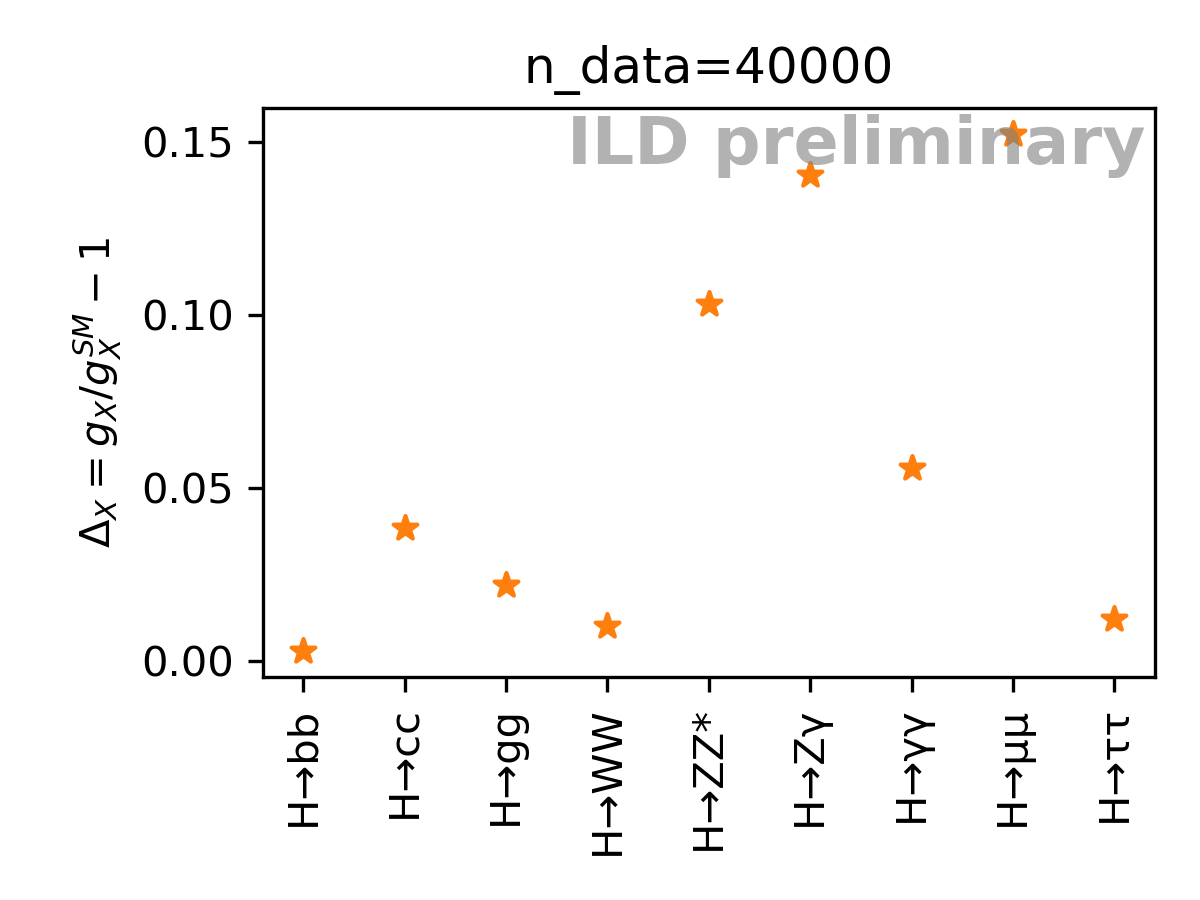
\includegraphics[width=0.8\textwidth, keepaspectratio]
      {plot_factory/br_relative_error}

  \end{column}
  \begin{column}{0.4\textwidth}
  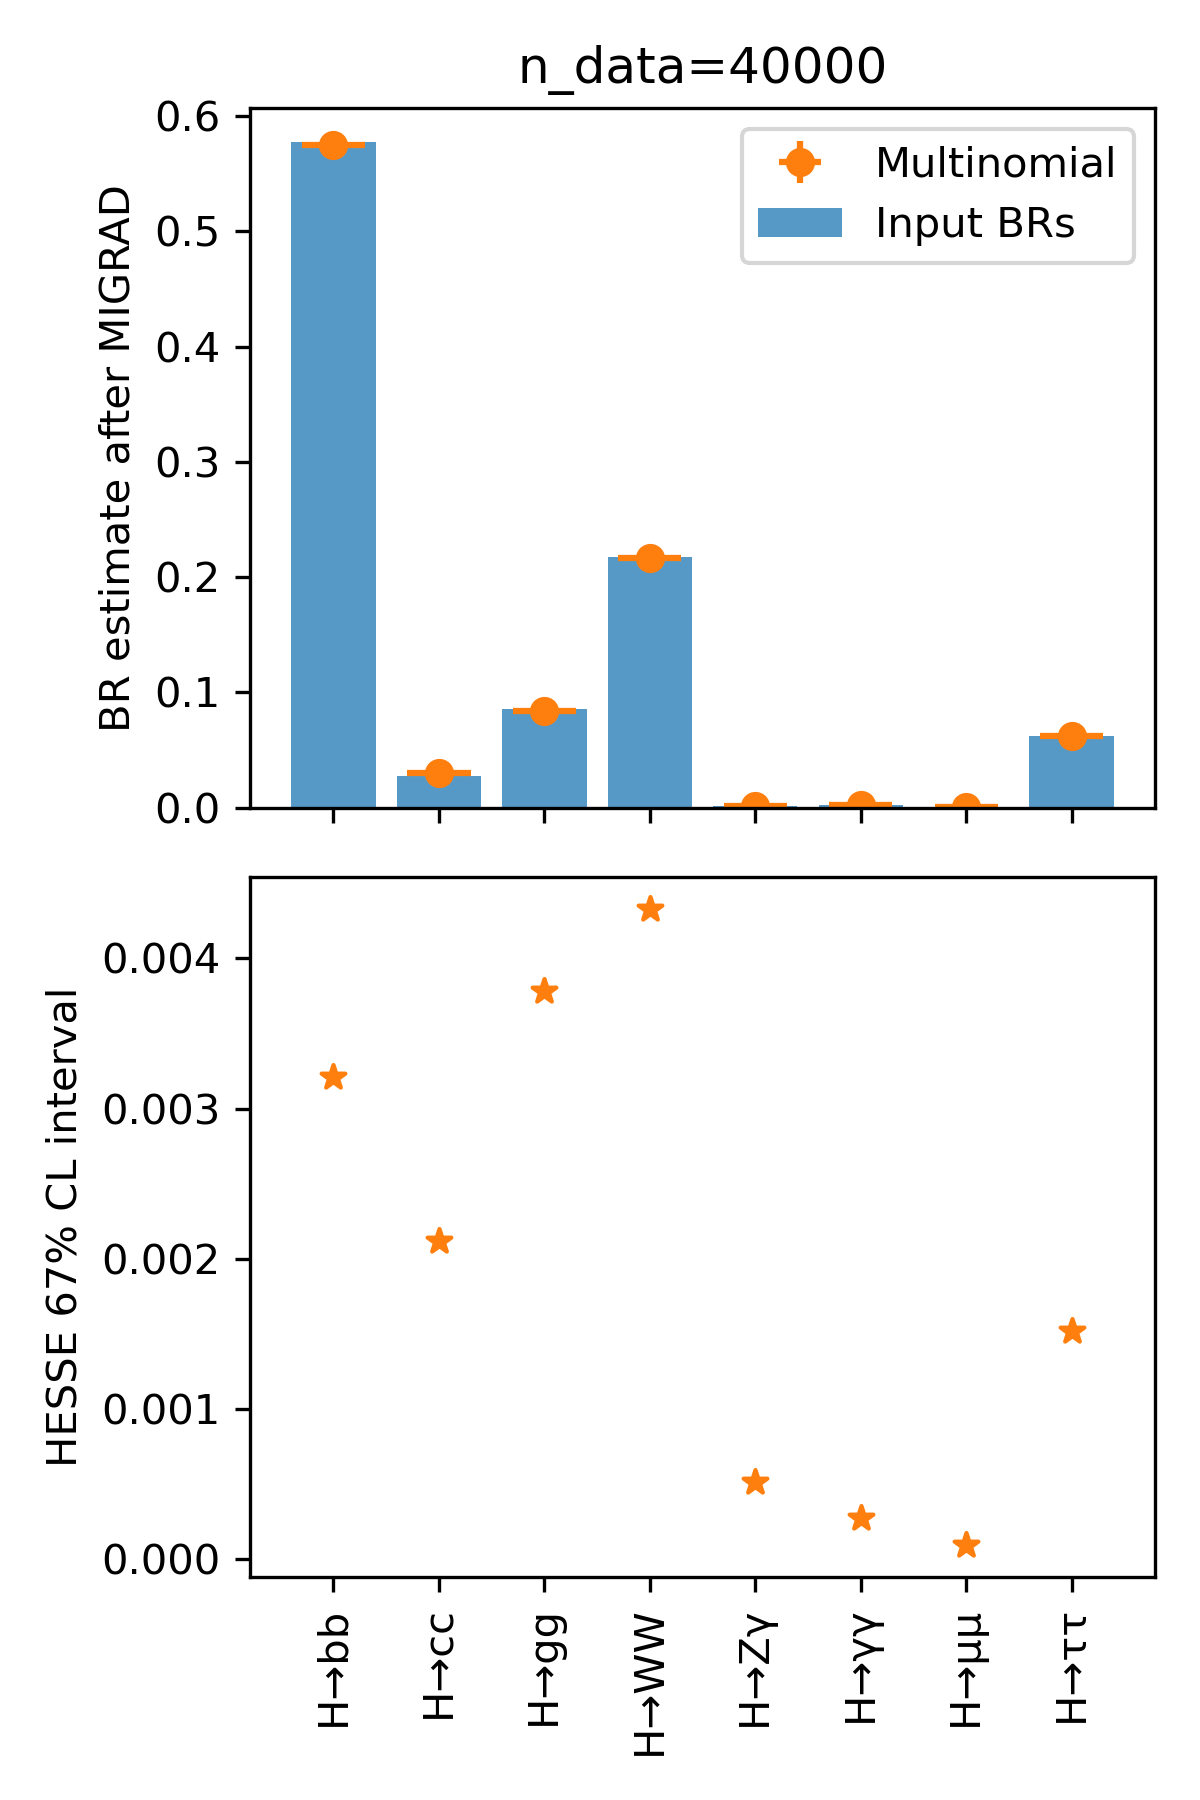
\includegraphics[height=0.99\textheight, width=0.95\textwidth, keepaspectratio]
      {plot_factory/br_estimates}
  \end{column}
  \end{columns}
  \end{frame}

\begin{frame}{Optimization - Results}
  \begin{columns}[c, onlytextwidth]
  \begin{column}{0.6\textwidth}
  Effect of the likelihood definition on the uncertainties.

  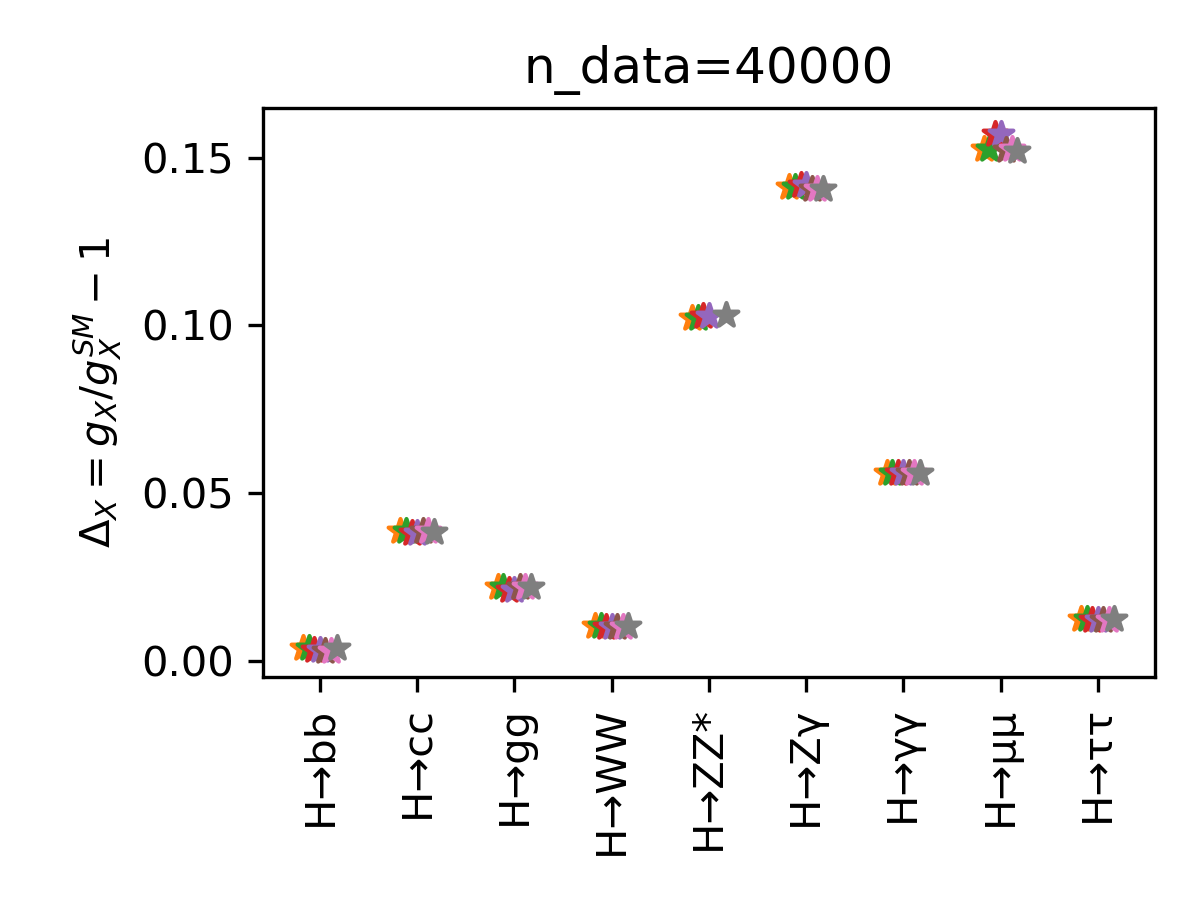
\includegraphics[width=0.8\textwidth, keepaspectratio]
      {plot_factory/many_br_relative_error}

  \end{column}
  \begin{column}{0.4\textwidth}
  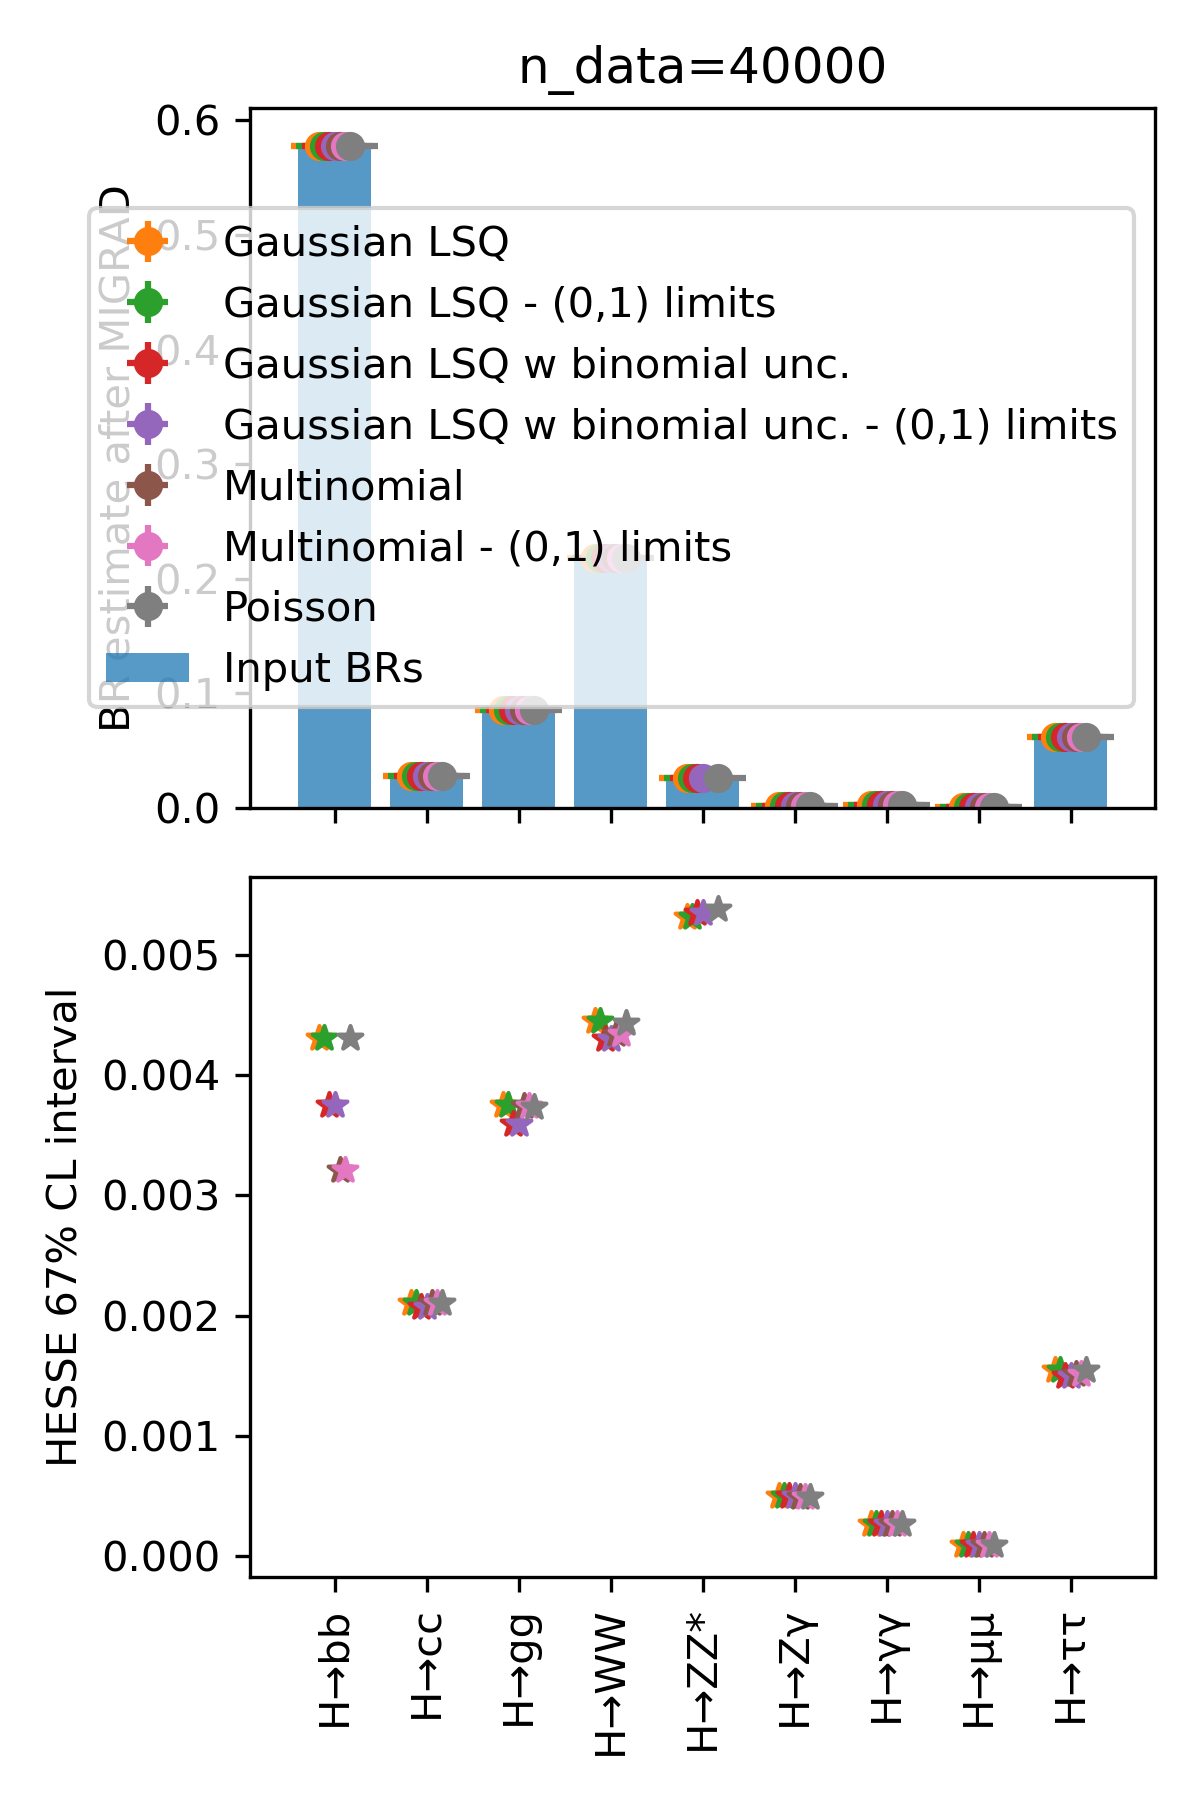
\includegraphics[height=0.99\textheight, width=0.95\textwidth, keepaspectratio]
      {plot_factory/many_br_estimates}
  \end{column}
  \end{columns}
  \end{frame}

\begin{frame}{Optimization - Validity check}
  Toy study: Draw from multinomial ($N_{\tn{data}}$ fixed).

  Shown: 2 of the toy fit distributions for multinomial $\tn{ln}\mathcal{L}$ with $\left[0, 1\right]$ boundaries.
  \begin{columns}[c, onlytextwidth]
  \begin{column}{0.5\textwidth}
  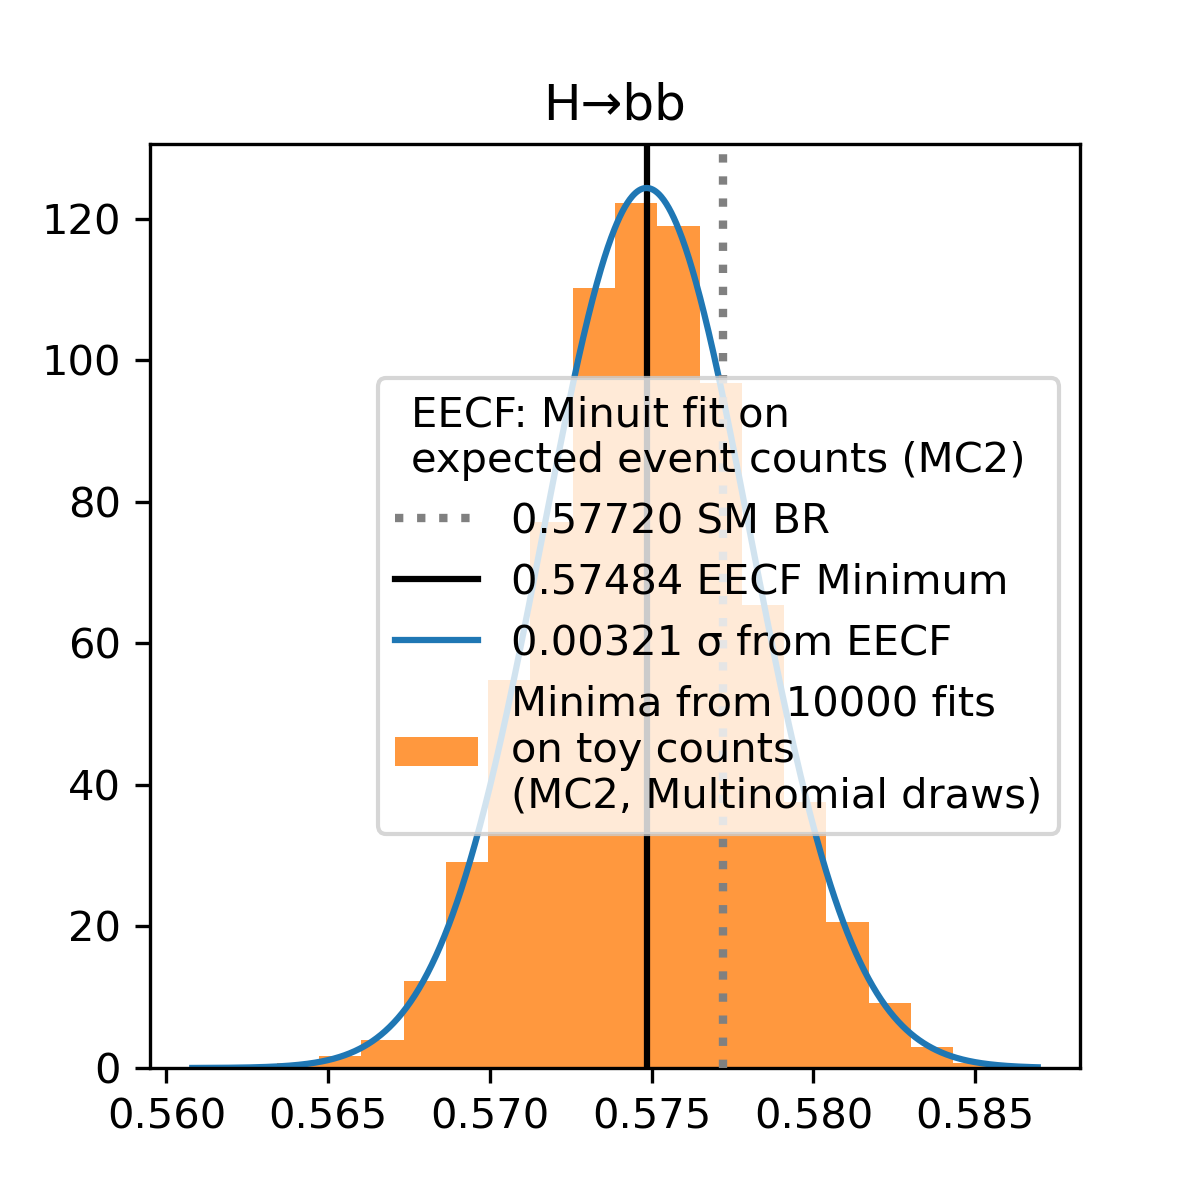
\includegraphics[height=0.7\textheight, keepaspectratio]
      {plot_factory/toys_multinomial/H_bb}
  \end{column}
  \begin{column}{0.5\textwidth}
  \includegraphics[height=0.7\textheight, keepaspectratio]
      {plot_factory/toys_multinomial/H_Zγ}
  \end{column}
  \end{columns}
  \end{frame}